\subsection*{Problema 03}

\textbf{Enunciado:} Calcular la integral:
\begin{equation*}
\int \frac{(2x-3)dx}{x^2 + 6x + 15}
\end{equation*}

\textbf{Solución:} Para resolver esta integral racional, analizamos el denominador $x^2 + 6x + 15$. Su derivada es $2x + 6$. 

Siguiendo la indicación, reescribimos el numerador de manera que aparezca la derivada del denominador, ajustando con una constante:
\begin{equation*}
2x - 3 = (2x + 6) - 9
\end{equation*}

Sustituimos esta expresión en la integral original y la separamos en dos integrales distintas:
\begin{align*}
I &= \int \frac{2x - 3}{x^2 + 6x + 15} \, dx \\
&= \int \frac{2x + 6}{x^2 + 6x + 15} \, dx \\
&\quad - \int \frac{9}{x^2 + 6x + 15} \, dx
\end{align*}

Para la primera integral, hacemos el cambio de variable $u = x^2 + 6x + 15$, cuyo diferencial es $du = (2x + 6)dx$:
\begin{align*}
I_1 &= \int \frac{2x + 6}{x^2 + 6x + 15} \, dx \\
&= \ln|x^2 + 6x + 15|
\end{align*}

Para la segunda integral, completamos el trinomio cuadrado perfecto en el denominador:
\begin{align*}
x^2 + 6x + 15 &= (x^2 + 6x + 9) - 9 + 15 \\
&= (x + 3)^2 + 6
\end{align*}

Reescribimos la segunda integral en función de esta forma estándar de arco tangente:
\begin{align*}
I_2 &= 9 \int \frac{dx}{(x + 3)^2 + 6} \\
&= \frac{9}{\sqrt{6}} \arctan\left(\frac{x + 3}{\sqrt{6}}\right)
\end{align*}

Combinando ambos resultados y añadiendo la constante de integración $C$, obtenemos la solución general:
\begin{align*}
I &= \ln(x^2 + 6x + 15) \\
&\quad - \frac{3\sqrt{6}}{2} \arctan\left(\frac{x + 3}{\sqrt{6}}\right) + C
\end{align*}

\begin{figure}[H]
	\centering
	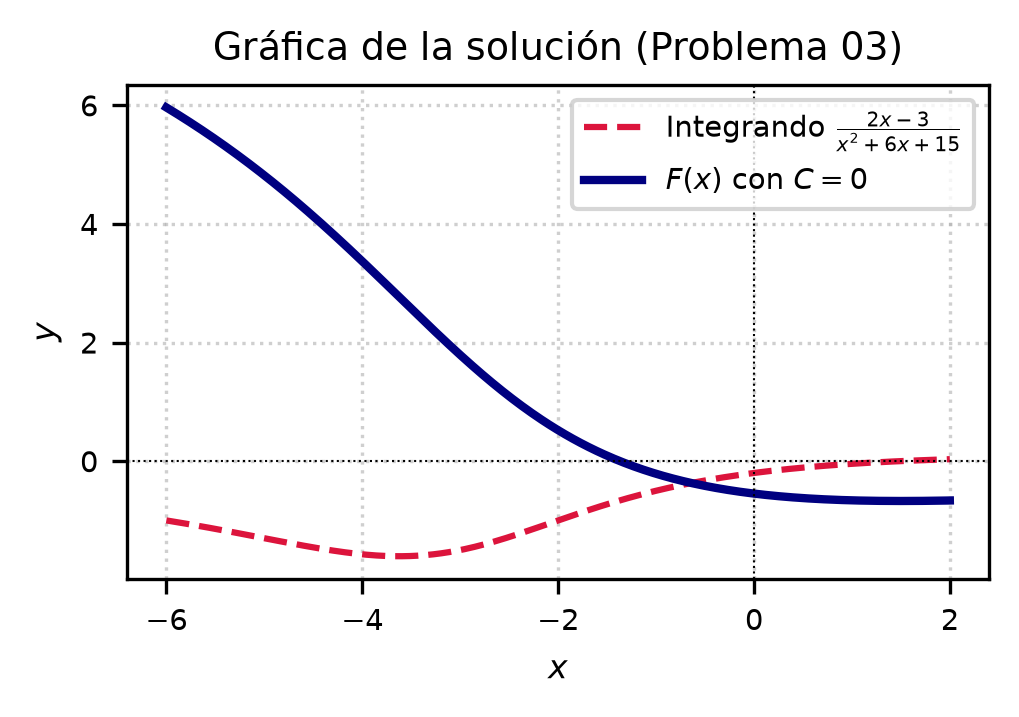
\includegraphics[width=\columnwidth]{semana_03/graficas/SEM03_P03_grafica.png}
	\caption{Representación gráfica de $f(x)$ y su antiderivada $F(x)$ evaluada para la constante de integración $C = 0$ (Problema 03).}
	\label{fig:problema03}
\end{figure}
